\begingroup
\setlength{\intextsep}{0pt}
\begin{figure}[H]
  \centering
  \captionsetup{skip=6pt}
  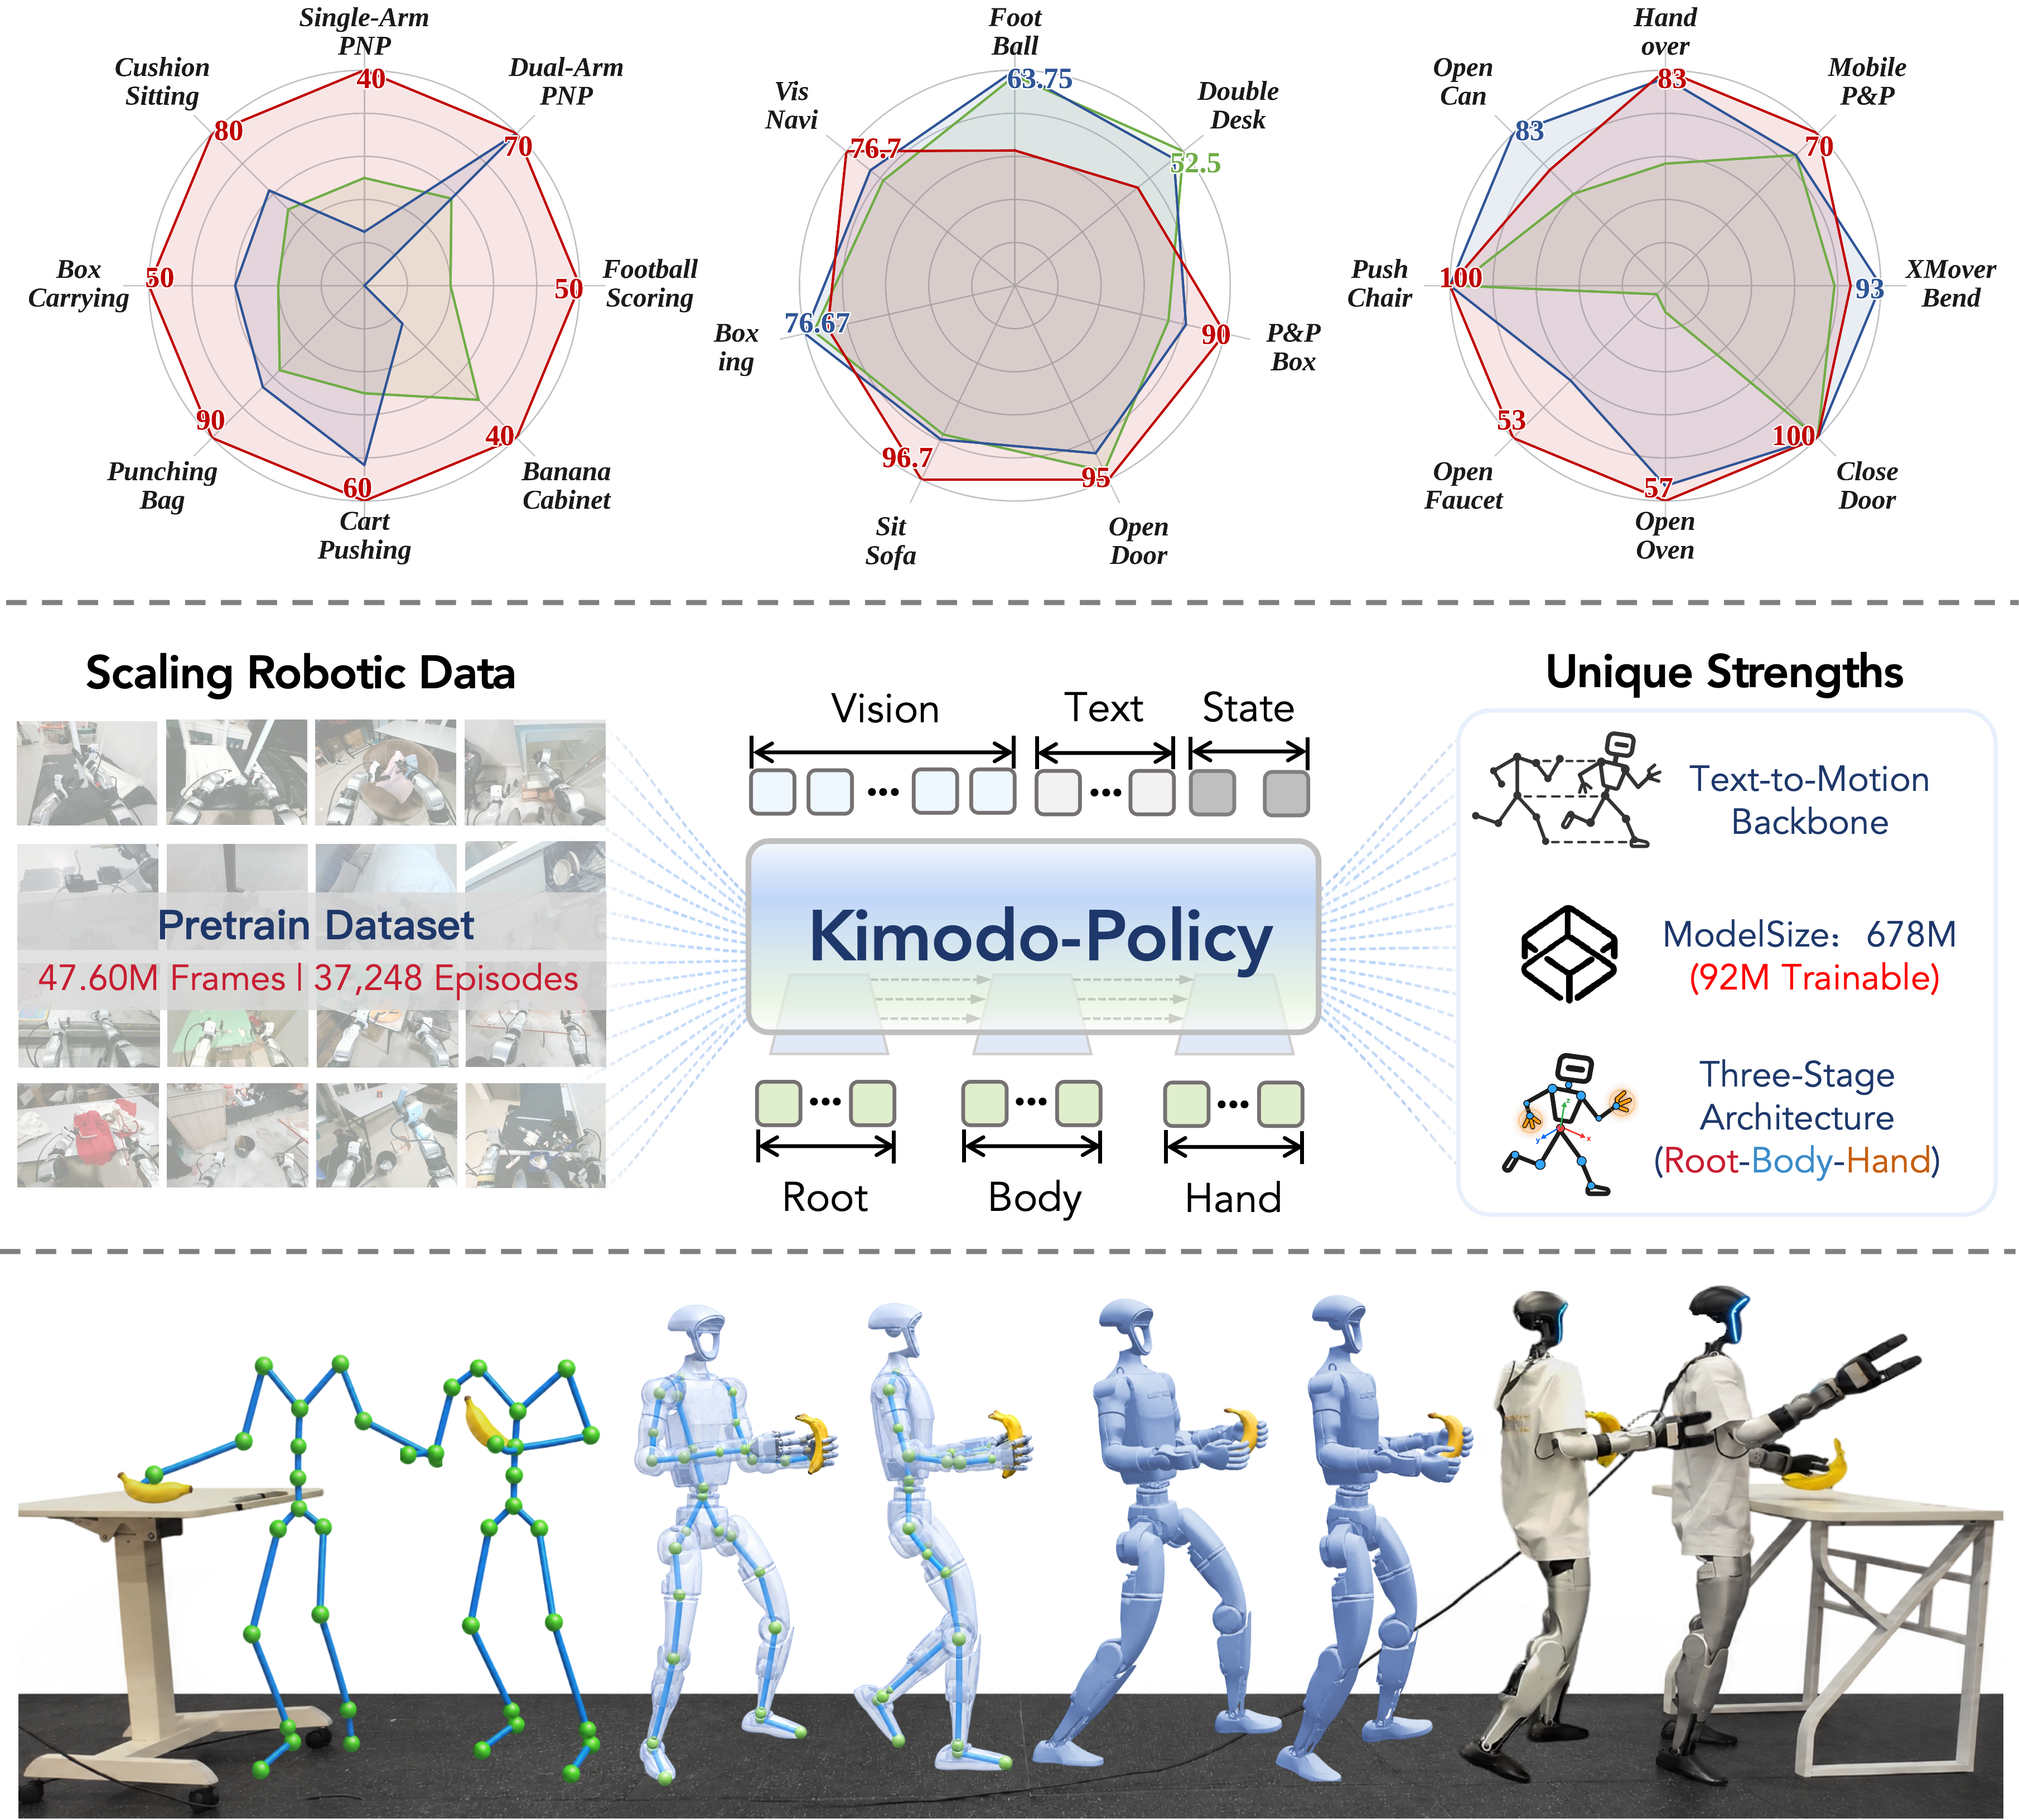
\includegraphics[width=\textwidth]{image/teaser.png}
  \caption{\textbf{Kimodo-Policy as an Instantiation of Kinematic Action Models (KAMs).}
  \textit{Top.} \inlinecolorblock{red!70!black}{red!70!black} Kimodo-Policy, \inlinecolorblock{blue!60!black}{blue!60!black} best baseline, and \inlinecolorblock{green!45!black!65!white}{green!45!black!65!white} second-best baseline. Our KAM-based policy achieves higher mean success than the evaluated VLA and WAM baselines on shared tasks.
  \textit{Middle.} Kimodo-Policy instantiates KAMs by inheriting whole-body motion priors from a pretrained motion generator. The compact policy (678M parameters, 92M trainable) combines large-scale loco-manipulation pretraining with a three-stage root--body--hand architecture.
  \textit{Bottom.} Observed motion history conditions future action-chunk generation for closed-loop control, as demonstrated in real-world object transfer.}
  \label{fig:overview}
\end{figure}
\endgroup

\begin{hclAbstract}
\noindent\textbf{Abstract.}\quad
Vision--language--action models and world action models transfer semantic and visual dynamics priors to robot control, yet humanoid loco-manipulation additionally requires tightly coupled coordination of locomotion, posture, and manipulation. We introduce \textbf{Kinematic Action Models (KAMs)}, a paradigm that uses pretrained motion generation models as the primary backbone for embodied action generation. Motion pretraining supplies reusable whole-body coordination and temporal structure, shifting policy learning toward grounding these priors in perceptual observations, task objectives, and robot state. We instantiate this paradigm with \textbf{Kimodo-Policy}, which combines a frozen Kimodo text-to-motion backbone with lightweight ControlNet-based visual adapters. A three-stage root--body--hand architecture couples global movement, body articulation, and hand control, while motion-history conditioning supports temporally consistent action-chunk generation for closed-loop execution. Large-scale loco-manipulation pretraining adapts the policy to diverse robot interactions. With 678M total parameters and 92M trainable, Kimodo-Policy achieves the highest overall success among evaluated policies on multi-task HumanoidArena (72.14\%), competitive performance on SIMPLE, and 60\% mean success across eight real-world tasks, outperforming the evaluated physical-robot baselines. Ablations support the contribution of motion pretraining, and matched-capacity comparisons show that the choice of motion prior affects downstream performance. These results establish Kimodo-Policy as an initial validation of KAMs for humanoid loco-manipulation.
\end{hclAbstract}
